% ****** Start of file apssamp.tex ******
%
%   This file is part of the APS files in the REVTeX 4.1 distribution.
%   Version 4.1r of REVTeX, August 2010
%
%   Copyright (c) 2009, 2010 The American Physical Society.
%
%   See the REVTeX 4 README file for restrictions and more information.
%
% TeX'ing this file requires that you have AMS-LaTeX 2.0 installed
% as well as the rest of the prerequisites for REVTeX 4.1
%
% See the REVTeX 4 README file
% It also requires running BibTeX. The commands are as follows:
%
%  1)  latex aps25samp.tex
%  2)  bibtex apssamp
%  3)  latex apssamp.tex
%  4)  latex apssamp.tex
%
\documentclass[%
 reprint,
nofootinbib,
%superscriptaddress,
%groupedaddress,
%unsortedaddress,
%runinaddress,
%frontmatterverbose,
%preprint,
%showpacs,preprintnumbers,
%nofootinbib,
%nobibnotes,
%bibnotes,
aps,
%pra,
%prb,
%rmp,
%prstab,
%prstper,
%floatfix,
]{revtex4-1}

\usepackage[utf8]{inputenc}
\usepackage[english]{babel}
\usepackage{dsfont}
\usepackage{amsmath}
\usepackage{ mathrsfs }
\usepackage{amssymb}
\usepackage{graphicx}% Include figure files
\usepackage{dcolumn}% Align table columns on decimal point
\usepackage{bm}% bold math
\usepackage{amsmath}
\usepackage{varioref}
\usepackage{booktabs}
\usepackage[bottom]{footmisc}
\usepackage{minted} % for pseudocode

\usepackage{physics}
\usepackage[ruled,vlined]{algorithm2e}
\usepackage{algpseudocode}
\usepackage{listings}

\usepackage{booktabs}

\usepackage{tikz}
\usepackage{float}
\usepackage{siunitx}



\newcolumntype{C}{>{$}c<{$}}
\AtBeginDocument{
\heavyrulewidth=.08em
\lightrulewidth=.05em
\cmidrulewidth=.03em
\belowrulesep=.65ex
\belowbottomsep=0pt
\aboverulesep=.4ex
\abovetopsep=0pt
\cmidrulesep=\doublerulesep
\cmidrulekern=.5em
\defaultaddspace=.5em
}

\newtheorem{theorem}{Teorem}
\usepackage{hyperref}% add hypertext capabilities
%\usepackage[mathlines]{lineno}% Enable numbering of text and display math
%\linenumbers\relax % Commence numbering lines

%\usepackage[showframe,%Uncomment any one of the following lines to test
%%scale=0.7, marginratio={1:1, 2:3}, ignoreall,% default settings
%%text={7in,10in},centering,
%%margin=1.5in,
%%total={6.5in,8.75in}, top=1.2in, left=0.9in, includefoot,
%%height=10in,a5paper,hmargin={3cm,0.8in},
%]{geometry}

% \renewcommand{\vec}[1]{\mathbf{#1}} %ny definisjon av \vec så det blir bold face i stedet for vector-pil.

\begin{document}


\title{En videnskablig analyse af den maritime tommelfingerregel for vurderingen af potentielle kollisioner ved betragtning af omgivelsernes relative bevægelse til det eventuelle kollisionsfartøj}
\author{Mikkel Metzsch Jensen}

\affiliation{Department of Physics, University of Oslo\\}
\date{\today}



\begin{abstract}
  Abstract
\end{abstract}

\maketitle
\newpage


\section{Introduktion}
Som søfarer findes der en lang række nødvendige og basale regler som sikrer orden og sikkerhed til søs. Dette er regler som indgår i duelighedsbevis for motor- og sejlbåd. Et af de mest centrale formål med disse regler er at undgå kollisioner mellem naturlige objekter eller andre fartøjer til søs. Reglerne beskriver hvordan søfaren skal agere i tilfælle af kollisionskurs, men det er essentielt at søfaren bliver opmærksom på denne kollisionskurs i så god tid som mulig.
% I sejlbåds regi bevæger fartøjet sig ofte med relative lave hastigheder, hvilket giver søfaren god chance for at korrigere ved eventuel kollisionskurs. Dog kan en sen reaktion blive farlig ved involvering af flere fartøjer og derfor er det fordelagtigt for bådføren at kunne korrigere for mulige kollisioner i god tid.
En forslået tommelfingerregel for denne vurdering bruger en betræktning af hvordan bagrunden flytter sig i forhold til et potentielt kollisionsfartøj. Ifølge \cite{duelighed} kan man ved "betydelige afstande" til kysten bruge observationen om hvordan kollisionsfartøjet trækker "over land" til at vurdere peilingen (Retning fra iagttageren til den genstand, der pejles \cite{ordbog}). Altså hævdes det at hvis den modsejlende trækker mod højre (styrbord) i forhold baggrunden så vil fartøjet gå højre om iagterens fartøj. Modsat vil det gå venstre (bagbord) om iagterens fartøj hvis det trækker til venstre over land. Hvis ikke fartøjet bevæger sig kendeligt i forhold til baggrunden, vil det efter sigende indikere at fartøjene på kollisionskurs. \\
En anden måde at vurdere pejlingen mere direkte er ifølge \cite{studienoter}, \cite{retsinformation} og \cite{groensund} ved at vurdere kollisionsfartøjets bevægelse relativt til et fast punkt på iagterens eget fartøj. Dette er en metode som hævdes at fastslå pejlingen uafhængig af afstanden til kysten \\
I denne rapport skal vi fremføre en matematisk analyse af pejlingens betydning for at vurdere kollisjonskurs. Med udgangspunkt i dette undersøger vi da om den såkaldte baggrundsmetode er en pålidelig metode til at pejlingen og dermed faren for kollision. \\
I denne rapport dækkes nogle af områdene dobbelt med brug af både matematisk notation og igen med mere letlæselig sproglig gengivelse af essensen. Dette gøres med tanke på at give en fuldkommen beskrivelse af problemet men samtidig også formidle det til folk uden speciale  forkundskaber i matematik og fysik.



\section{Metode}
\subsubsection{Definering af problemet}
Vi forestiller os to både til søs, som nærmer sig hinanden. Vi kalder den ene båd for hovedbåden (HB), hvor vi har placeret iagtageren, som ønsker at vurdere om bådene er på kollisionskurs. Den anden båd kalder vi for kollisionsbåden (KB). Vi antager at begge bådene bevæger sig med konstant hastighed, dvs. retlinjet og med konstant fart. For enkelthedes skyld antager vi at bådene kan reduseres til et enkelt punkt i et to-dimensionsjonalt aksesystem som tilsvarer bådens position på vandets overflade. Vi bruger aksetitlerne x og y til at beskrive positionen $\vec{P} = (x, y)$ . Positionen til hver båd bliver da en funktion af tid bestemt af parametrene: Startposition $\vec{P}_0$ og hastighed $\vec{v}$. For de to både følger bevægelseslingingen
\begin{align*}
  \vec{P}(t) =  \vec{P}_0 + \vec{v}\cdot t
\end{align*}
Vi definerer en kollision ved at bådene har samme position ved samme tidspunkt. \\
For at vudere om bådene er på kollisionskurs er det angiveligt nyttigt at benytte pejlingen. Vi definerer i matematisk forstand pejlingen $\theta_{HB}$ fra HB som vinklenen mellem kursen til HB og sigtelinjen fra HB til KB. Dette er illustreret på figur X. (INDSÆT BILLEDE)







\section{Resultater}

\subsection{Pejlingens betydning for kollisionskurs}
Siden vi antager at bådene bevæger sig med konstant hastighed kan vi bruge en lineær transformation til at skifte koordinatsystem til intertialsystemet hvor HB er i ro (HB's intertialsystem). Med andre så kan vi frit vælge at beskrive positionen til KB som den opleves for en iagtager ombord på HB. Positionen $P'_{KB}$ til KB i det nye intertialsystem kan skrives:
\begin{align*}
  \vec{P'}_{KB}(t) &= \vec{P}_{KB}(t) - \vec{P}_{HB}(t) \\
  &= \vec{P}_{0,KB} + \vec{v}_{KB}t - \vec{P}_{0,HB} - \vec{v}_{HB}t \\
  &= (\vec{P}_{0,KB} - \vec{P}_{0,HB}) + (\vec{v}_{KB} - \vec{v}_{HB})t \\
  &= \vec{P'}_{0,KB} + \vec{v'}_{KB}t
\end{align*}
Vi ser at $P'_{KB}$ også beskriver en retlinjet bevægelse. I tilfællet hvor bådene er på kollisionskurs ved vi at $P'_{KB}(t_k) = 0$ ved kollisionstidspunktet $t_{k}$. Dette medfører sammenhængen:
\begin{align}
  \vec{P'}_{0,KB} &= - \vec{v'}_{KB}t_k \nonumber \\
  \begin{pmatrix} x'_{0,KB} \\ y'_{0,KB} \end{pmatrix}\frac{1}{t_k} &=   -\begin{pmatrix} v'_{x,KB} \\ v'_{y,KB} \end{pmatrix}
  \label{eq:P=v}
\end{align}
Vi kan da finde pejlingen $\theta_{HB}$ via ved at omrksive $P'_{KB}$ til polære koordinater. Her er vi bare interesseret i vinkelkoordinat $\phi_{KB}$ som vi kan bestemmes som
\begin{align*}
  \phi_{KB}(t) &= \arctan{\left( \frac{y'(t)}{x'(t)}\right)} \\
  &= \arctan{\left( \frac{y'_{0,KB} + v'_{y,KB}t}{x'_{0,KB} + v'_{x,KB}t}\right)}
\end{align*}
Vi bruger da sammenghængen fra ligning \ref{eq:P=v} og finder
\begin{align*}
  \phi_{KB}(t) &= \arctan{\left( \frac{y'_{0,KB} - y'_{0,KB}\frac{t}{t_k}}{x'_{0,KB} - x'_{0,KB}\frac{t}{t_k}}\right)} \\
  &= \arctan{\left(\frac{y'_{0,KB}}{x'_{0,KB}} \frac{1 - \frac{t}{t_k}}{1 - \frac{t}{t_k}}\right)} \\
  &= \arctan{\left(\frac{y'_{0,KB}}{x'_{0,KB}}\right)} = \text{konst.} \\
\end{align*}
Fra dette ser vi at vinkelkoordinat $\phi_{KB}$ er konstant (uavhængig af tid) hvilket medfører at pejlingen også er konstant:
\begin{align*}
  \theta_{HB} &= \frac{\pi}{2} - \phi_{KB} = \text{konst.}
\end{align*}
Fra dette ræsonoment har vi altså vist at pejlingen vil være konstant i tilfællet hvor bådene er på kollisionkurs. Hvis bådene følger kollisionskursen men i modsat retning (bevæger sig væk fra hianden), kan vi indføre betingelsen $P'_{KB}(t_i) = 0$ for et tidspunkt $t_i < 0$. Derved kan vi opstille en ligning analog til \ref{eq:P=v} og derved finde at pejlingen også vil være konstant i dette tilfælle. Hvis ikke bådene er på kollisionskurs er ligning \ref{eq:P=v} ikke længere gyldig og $P'_{KB}$ kan tage hvilken som helst retlinjet bane. Det betyder at $\phi_{KB}$ og dermed også at pejlingen $\theta{KB}$ ændre sig som funktion af tid. Dette fører til slutningen:
% \begin{quote}
% Hvis og bare hvis bådene nærmer sig i afstand og har kollisionskurs vil pejlingen fra den ene båd til den anden være konstant.
% \end{quote}
\begin{theorem}
  Hvis og bare hvis to både har kollisionskurs og nærmer sig i afstand vil pejlingen fra den ene båd til den anden være konstant.
  \label{Teo:pejling}
\end{theorem}
\subsubsection{Gengivelse af konstant-pejling-udledningen uden matematisk notation}
Siden begge bådene antages at bevæge sig med konstant fart og i en ret linje vil en iagtager på HB også se at KB bevæger sig med konstant fart og i en ret linje. I tilfællet hvor bådene er på kollisionskurs vil en iagtager på HB se at KB har kurs direkte mod iagteren. Dette er den eneste måde at KB kan kollidere med HB under antagelsen om at fart og retning er konstant. Derfor følger det at pejlingen også vil være konstant i tilfællet med kollisionskurs.


% Kort sagt: bådene må bevæge sig på en ret linje, og hvis vi har to punkter kan vi tegne denne rette linje. Siden det ene punkt i kollision må den rette linje gå ud fra HB og derfor er pejlingen konstant.

 % vil det i begge koordinatsystemer have same position ved kollisionstidpunket. Siden KB bevæger sig med konstant hastighed ved vi at KB også har en retlinjet bevægelse i HB's intertialsystem. Derfor er det klart at bevægelsen til KB i HB's intertialsystem vil være en ret linje med endepunkt i HB's position. Dette medfører at pejlingen vil være konstant under hele bevægelsen. Bemærk at vi fortsat kan bruge kursretningen som referense til vinklen som bestemmer pejlingen selvom vi bruger HB's intertialsystem. Vi kan også have en situation hvor KB bevæger sig på en ret linje væk fra HB i HB's intertialsystem, hvilket naturligvis ikke vil opfylde kollisionsbetingelsen. Fra dette kan vi slutte at dersom pejlingen ikke ændres og afstanden mellem bådene bliver mindre, så er disse på kollisionskurs. Siden det fremstår trivielt at bedømme hvorvidt KB bevæger sig mod eller væk fra HB er det bestemmelsen af pejlingen som er afgørende for vurderingen af risikoen for kollision.


 \subsection{Grænsebetingelser for brug af kystens relative bevægelse som indikator}
 Med udgangspunkt i teorem \ref{Teo:pejling} kan vi undersøge hvorvidt brugen af baggrundens relative bevægelse kan bruges som en pålidelig indikator for en fremtidig kollision. Vi antager at den nærliggende kystlinje er retlinjet. I tilfællet med kollisionskurs ved vi fra teorem \ref{Teo:pejling} at sigtelinjen fra HB gennem KB vil have en konstant vinkel i forhold til kystlinjen. I det enkle tilfælle hvor kystlinjen er parallel med kursen til HB vil sigtelinjens skæring med kystlinjen flytte sig med samme hastighed som HB. Altså vil baggrunden bag KB set fra HB's perspektiv flytte sig på trods af at bådene er på kollisionskurs. Dette bekræftes ved simuleringen vist på figur \ref{fig:eks1}.
 \begin{figure}[H]
   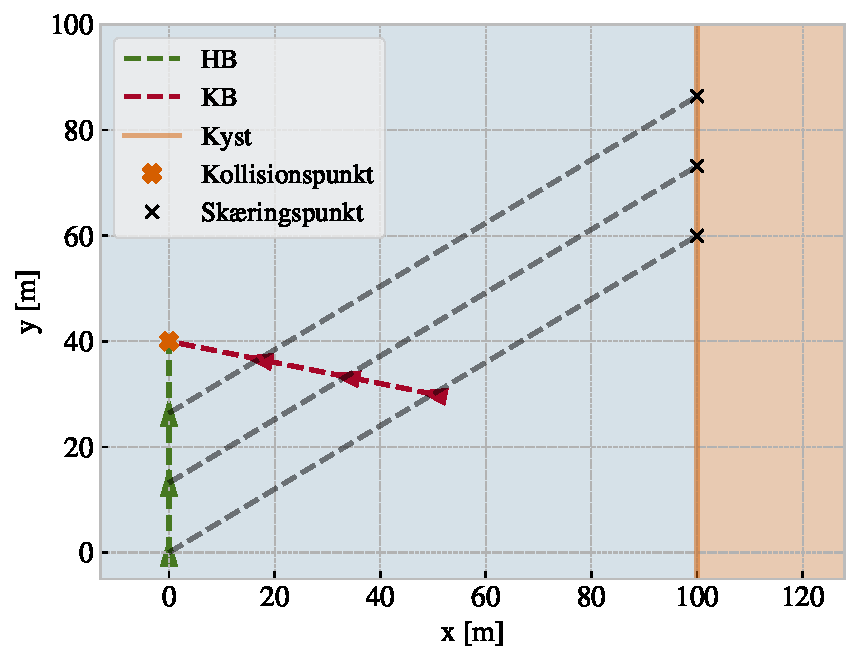
\includegraphics[width=\linewidth]{figures/eksempel1.pdf}
   \caption{En simulering af bådene HB og KB på kollisionskurs, med kollisionspunkt 100 meter fra kysten. Her plottes fire positioner for bådene (inklusiv kollisionspunktet) jævnt fordelt i tid. Fra de sorte stiblede linjer ser vi hvordan sigtelinjen fra HB gennem KB skærer med kysten. Dette skæringspunkt forflytter sig som forventet i henhold til HB's bevægelse.}
   \label{fig:eks1}
 \end{figure}
 Hvis kystlinjen ikke er parallel med kursen til HB vil afstanden mellem skæringspunkterne være større, mens vinkelen mellem de to punkter vil være det samme (Vis dette?).\\
 Hvis skæringspunktets forflytning er kendelig selvom bådene er på kollisionskurs vil dette medføre at baggrundsmetoden ikke er pålidelig i et sådan tilfælde.
 % Mulige faktorer som kan afgøre dette er hastigheden til HB, afstanden til kysten og vinkelen mellem kystlinjen og den direkte linje fra kyst til HB. \\

 \subsubsection{Definering af kendelig forflyting}
 For at vurdere hvorvidt baggrundsmetoden kan anvendes må vi definere hvad en kendelig forflytning er. Det meneskelige øje har en vinkelopløsning på 1 arcminut (ca. 0.02$^{\circ}$) hvilket tilsvarer 30 cm fra en afstand af 1 km \cite{wiki:eye}. Det betyder strengt taget at vi kan skelne mellom objekter som er plaseret 30 cm fra hinanden set fra 1 km afstand. Dette er dog ikke så relevant for kendelig hastighed? \\
 \\
 Vi kan antage at vi iagtager bådens relative bevægelse i forhold til KB over 5 sekunder. Naturlig vil man da benytte et centralt punkt på båden som referance punkt for samnmenligning med baggrunden. Vi siger da at hvis dette baggrundspunktet har flyttet sig ud over bådens udstrækning i løbet af de 5 sekunder, så er forflytningen kendelig. Det vil sige at punktet har forflyttet sig med en relativ hastighed på en halv bådlængde/bådbredde pr. 5 sekunder. Vi bruger at den effektive bådlængde er 8 meter. Vi kan antage at båden befinder sig omtrent 200 meter væk ved vurderingen, hvilket giver en vinkelhastighed $\omega$ på
 \begin{align*}
   \omega = \frac{\arctan{(\frac{4 \text{m}}{200 \text{m}})}}{5 \text{s}} \approx 0.004 s^{-1} = 0.2^{\circ}s^{-1}
 \end{align*}

 \subsubsection{Hvis at kystvinkel er irrelevant}



\subsection{Resultat for grænse}
forflytning $s$, afstand til kyst via sigtelinjen $d$ og bådhastighed parallel med kysten $v_{t}$ . Kriterium for brug af regel
\begin{align*}
  v_t &\le d\sin{(\omega)} \\
  \frac{v_t}{\sin{(\omega)}} &\le d \\
  \frac{v_t}{0.004}&\lesssim d
\end{align*}
En typisk bådhastighed kan være 4 knob hvilket tilsvarer omtrent 2 m/s. Indsætter vi dette i kriteriumet får vi
\begin{align*}
  500 \text{m} &\lesssim d
\end{align*}

\subsubsection{Modbevis af baggrundsmetoden}
\subsubsection{Sammenfald mellem baggrundsmetode og lokalt pejlemærke}

\section{Diskussion}

Bemærk at vi i praksis må tage hensyn til at båden har en hvis udstrækning og at den dermed også kolliderer når punkterne passerer tæt forbi hinanden. Dette har dog ikke betydning for den teortiske model, og ved andvendelse af modellen i praksis må man bruge resultaterne i overensstemmelse med en ønsket sikkerhedsradius ved forbipassering. (Se diskussion for mere info om dette.)


\section{Konklusion}

\begin{thebibliography}{}
  \bibitem{duelighed} Duelighed.dk. Date. Edition. Skipper-kursus (slide 03-02), tilgængelig ved \url{http://www.duelighed.dk/tutorial_soevejsregler/03_02.htm} (sidst læst: 05/01/2021)
  \bibitem{ordbog} Hjemmeværnet: Maritime udtryk, tilgængelig ved \url{https://www.hjv.dk/oe/HVF122/Sider/Maritime-udtryk.aspx} (sidst læst: 05/01/2021)
  \bibitem{studienoter} Søren Toftegaard O. (2013), \textit{LystSejlads}, s. 19 (afsnit 1.4) , tilgængelig ved \url{http://studienoter.dk/Sejlads/Noter/LystSejlads.pdf} (sidst læst: 05/01/2021)
  \bibitem{retsinformation} retsinformation.dk: \textit{Bekendtgørelse om søvejsregler} 20/11/2009. Regel 7: fare for sammenstød (d) (20/11/2009), tilgængelig ved \url{https://www.retsinformation.dk/eli/lta/2009/1083} (sidst læst: 05/01/2021)
  \bibitem{groensund} Albrechten S. (2007). \textit{Sejlads for Begyndere} \url{http://www.groensund.dk/upl/website/sejlads/SejladsforBegyndere2.pdf}
  \bibitem{wiki:eye} Wikipedia: Naked eye \url{https://en.wikipedia.org/wiki/Naked_eye} (sidst læst: 11/01)
\end{thebibliography}

\section*{Appendix}
\subsection{Plots for simuleringer der bekræfter det matematiske teorem}


%\bibliographystyle{plain}

\end{document}
